\documentclass[8pt]{extarticle}
\usepackage{makeidx}
\usepackage{graphicx}
\usepackage{amsmath}
\usepackage{amssymb}
\usepackage{latexsym}
\renewcommand\refname{Referenze}
\usepackage[utf8x]{inputenc}
\usepackage{titlesec}
\usepackage{bm}
\usepackage{mathtools}
\usepackage[document]{ragged2e}
\titleformat{\section}{\huge\normalfont\bf}{\thesection.\hspace{5pt}}{5pt}{\vspace{1cm}}
\titleformat*{\subsection}{\Large\bfseries}
\usepackage[inner=3cm,outer=3cm]{geometry}

\makeindex

\begin{document}
\justify
\printindex
\Large{A.a. 2013-2014}
\vspace{10cm}
\begin{center}
\Huge\textbf{Analisi Dati}
\end{center}

\vspace{2cm}
\begin{flushleft}
\textit{Gruppo \textsc{1}} \\
\medskip
Federico \textsc{Massa} \\ 
Marco \textsc{Montella}
\end{flushleft}



\newpage

\begin{abstract}
\justify
 

\end{abstract}
\bigskip

\section{Introduzione} \label{sec:intro}
Scopo dell'esperimento è determinare la frazione di mesoni K in un fascio monocromatico contenente K e $\pi$ analizzando i dati di una simulazione del passaggio di quest'ultimo attraverso un apparato sperimentale composto da un rivelatore Cerenkov a gas e uno scintillatore posto a valle. Alla frazione di K nel fascio si deve inoltre correlare un intervallo di confidenza sul raggio degli anelli Cerenkov prodotti nel rivelatore e in relazione ad esso determinare la probabilità di non identificare un evento legittimo di K e di accettare come K un evento dovuto ad un $\pi$. \\
Analizzando i medesimi dati si deve inoltre determinare l'indice di rifrazione del gas contenuto nel rivelatore Cerenkov. \\

L'effetto Cerenkov, consiste nel rilascio di luce visibile o ultravioletta all'interno di un materiale (solitamente gassoso o liquido) quando esso viene attraversato da una
particella la cui velocità è superiore alla velocità della luce nel mezzo.\\
Come risultato dell'interazione con il mezzo viene rilasciato un cono di luce con vertice nella posizione della particella e apertura angolare funzione della velocità della particella e dell'indice di rifrazione del mezzo.\\
Essendo il coseno di theta una funzione limitata, fissato un indice di rifrazione si avrà rilascio di fotoni solamente per un determinato intervallo di valori di $\beta=v/c$, il che rende possibile utilizzare i rivelatori Cerenkov come rivelatori a soglia in eventuali misure di veto.
I rivelatori Cerenkov sfruttano tale effetto rivelando i fotoni emessi grazie ad una apposita superficie otticamente attiva sulla superficie interna o su una delle basi, quest'ultimo il caso dell'apparato considerato nella presente analisi.
% Il rivelatore cerenkov che si prende in considerazione in questa analisi è dotato, sulla base più lontana relativamente al verso delle particelle del fascio, di uno specchio parabolico la cui lunghezza focale è pari alla lunghezza del rivelatore. Sulla base opposta, in corrispondenza del piano focale, si trova un rivelatore a pixel 50x50 di dimensioni 1cmx1cm. Lo specchio parabolico ha la proprietà di "focalizzare" fasci di luce paralleli su un punto del piano focale funzione dell'angolo formato dal fascio con l'asse ottico, sebbene solo quando questo angolo è zero la messa a fuoco risulta priva di aberrazione. Sulla base otticamente sensibile i pixel interessati dall'arrivo di uno o più fotoni formeranno dunque, a causa della simmetria sull'angolo azimutale, di un anello il cui raggio può essere messo in relazione con l'angolo di emissione dei fotoni, e di conseguenza con la velocità della particella. 
A partire quindi dalle informazioni sulle regioni della superficie attiva interessate dalla luce Cerenkov, è possibile, in un fascio monocromatico composto da particelle di diverso, sfruttare la relazione tra angolo di emissione e massa delle varie specie di particelle per identificare e quantificare le varie componenti del fascio.

\section{Apparato}
L'apparato sperimentale simulato consiste di un rivelatore Cerenkov a gas di indice di rifrazione $n$ ignoto da determinarsi nell'analisi, di lunghezza $1000 \ cm$, pari alla lunghezza focale dello specchio parabolico posto sul fondo del recipiente contenente il gas. Il rivelatore a di fotoni Cerenkov posto sul piano focale dello specchio è un quadrato composto da 2500 pixel ciascuno di dimensioni $1 \ cm$ x $1 \ cm$. \\
\subsection{Formazione degli anelli Cerenkov}
Al passaggio di una particella con $\beta > c/n$, si ha nel gas un'emissione di fotoni visibili o ultravioletti ad un angolo $\theta$ con la direzione del fascio per cui vale:
\begin{equation} \label{eq:cerenkov}
\cos{\theta}=\frac{1}{\beta n}
\end{equation}
Il fotone raggiunge lo specchio parabolico e viene riflesso producendo, a meno di inefficienze nella riflessione, nella trasmissione nel gas o nella rivelazione, un segnale in uno dei pixel. Essendoci una simmetria sull'angolo azimutale $\phi$, l'insieme di tutti i fotoni che possono essere emessi dalla particella a una distanza $d$ fissata dal vertice dello specchio forma una circonferenza sul piano focale.\\
\'E possibile dimostrare che il raggio di tale circonferenza è indipendente dal punto di emissione $d$, e che pertanto tutti i fotoni emessi dalla particella nel suo percorso all'interno della camera a gas vengono messi a fuoco su una circonferenza il cui raggio dipende solamente dall'angolo Cerenkov e dalle caratteristiche dello specchio parabolico.\\
Chiamando $\theta$ l'angolo Cerenkov, $d$ la distanza di emissione dal vertice della parabola, $f$ la distanza focale, $\delta$ l'angolo formato dalla tangente alla parabola nel punto di riflessione del fotone con un asse parallelo al piano focale e $x0$ la distanza del punto di riflessione dal vertice della parabola lungo l'asse di quest'ultima, il raggio $R$ dell'anello Cerenkov risulta:
\begin{equation} \label{eq:raggio_theta}
R \ = \ \frac{f+x_0 \cot{\theta}+x_0 \cot{(\theta-2\delta)}-d}{\cot{(\theta-2\delta)}}
\end{equation}
\begin{equation}
x_0 \ = \frac{f}{2} \Bigg[-\cot{\theta}+\sqrt{\cot{\theta}^2+\frac{d}{f}}\ \Bigg] \ \ \ \ \ \ \ \tan{\delta}=\frac{2x_0}{f}
\end{equation}
La relazione \eqref{eq:raggio_theta} è stata codificata in ROOT ad angolo fissato pari a $1.47 °$, valore che, come si vedrà, corrisponde all'angolo che i fotoni Cerenkov dei $\pi$ formano col fascio. Nella figura \ref{fig:tf1_ringdistance} è mostrato l'andamento del raggio con la distanza di emissione.\\

\begin{figure}
\begin{center}
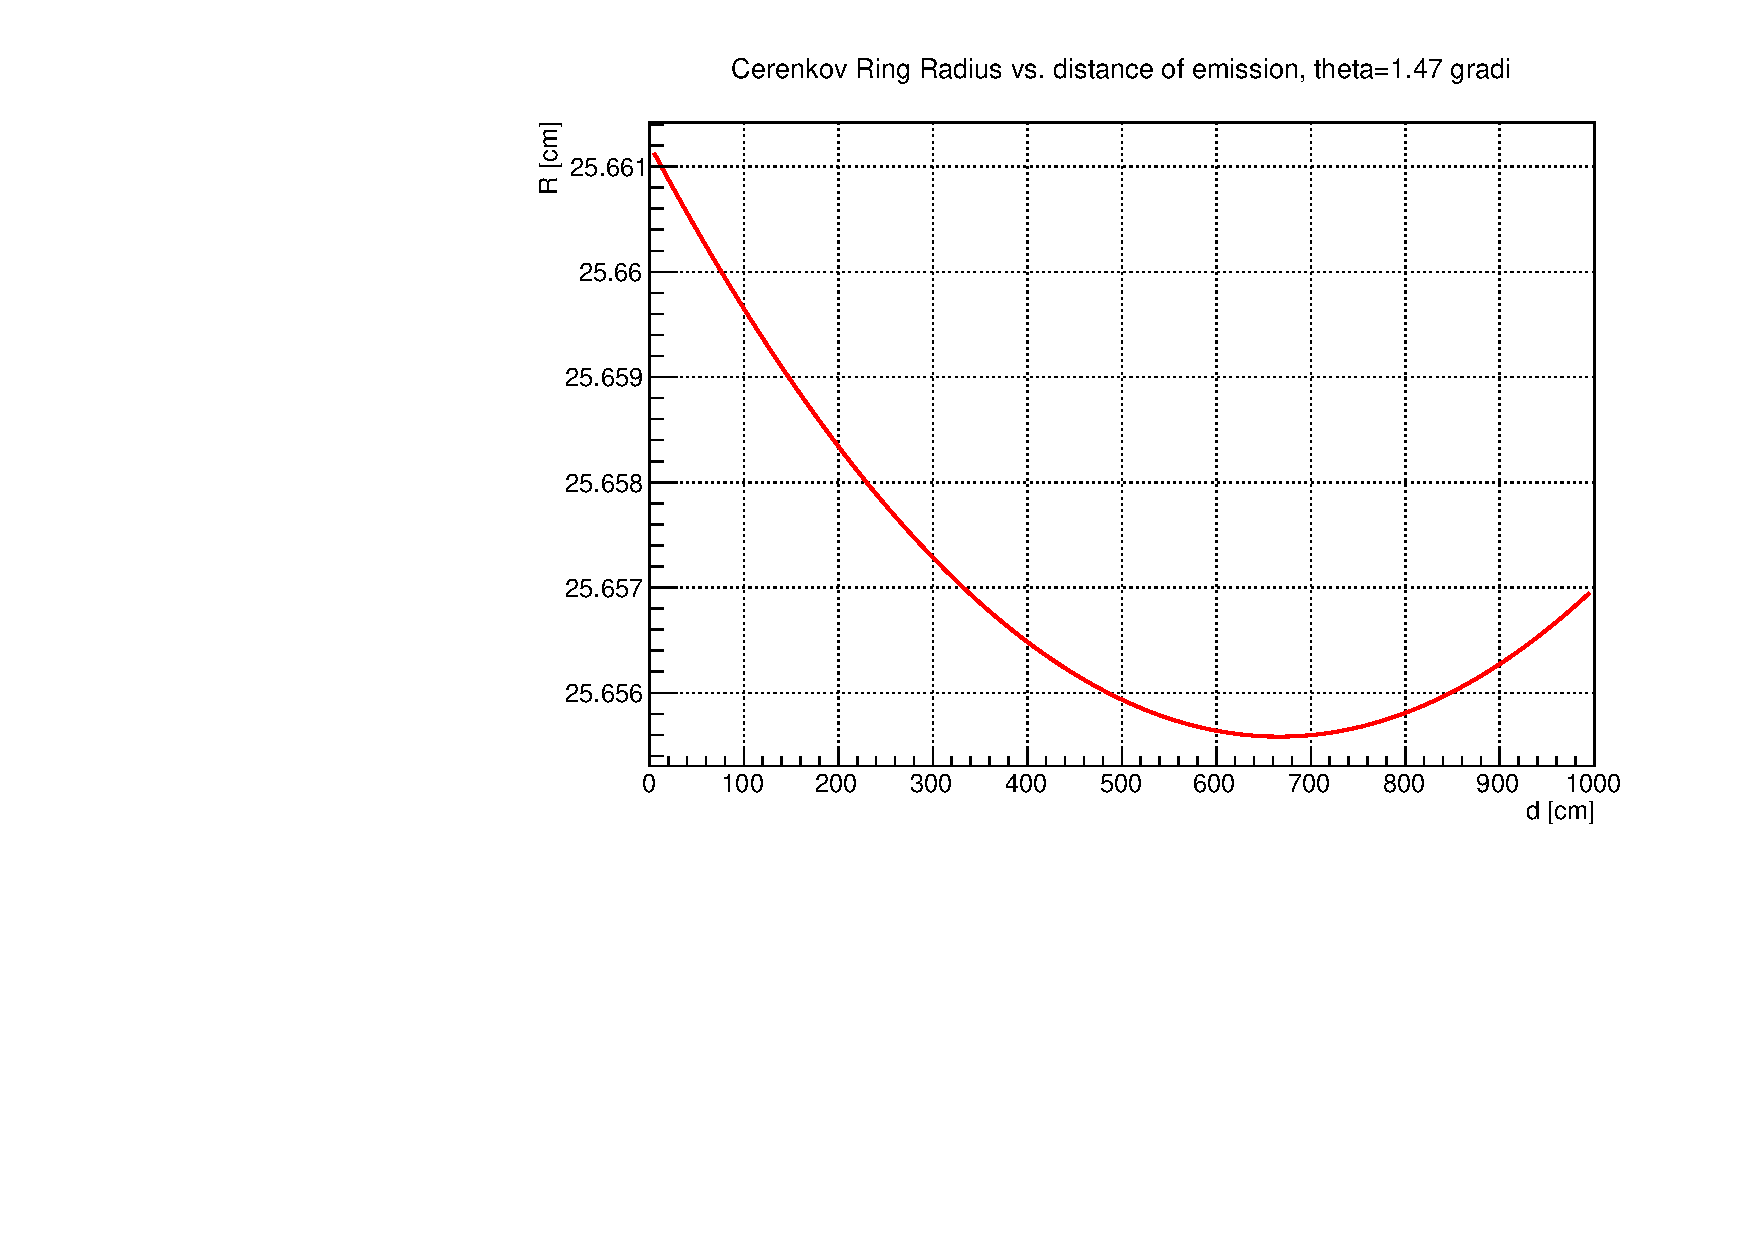
\includegraphics[scale=0.4]{tf1_ringdistance}
\caption{Relazione tra il raggio e la distanza di emissione per un fotone Cerenkov prodotto a 1.47° rispetto al fascio. La distanza massima corrisponde alla dimensione del rivelatore Cerenkov.}
\label{tf1_ringdistance}
\end{center}
\end{figure}

La non costanza del raggio in funzione di d è dovuta al fatto che uno specchio parabolica è in grado di mettere a fuoco solamente raggi paralleli all'asse ottico. L'aberrazione sulle immagini provenienti da sorgenti fuori asse è nota come \textit{coma}.
Ad ogni modo lo scarto relativo tra gli estremi di variabilità del raggio è dell'ordine di $10^{-4}$, ed è trascurabile rispetto all'incertezza derivante dalla discretizzazione delle posizioni dei punti sperimentali introdotta dai pixel, dell'ordine quest'ultima di $4\cdot 10^-2$.\\
Le figure \ref{fig:tf2_radius} e \ref{fig:tf2_radius_zoom} mostrano invece l'andamento del raggio in funzione contemporaneamente di $\theta$ e $d$. 
\begin{figure}
\begin{center}
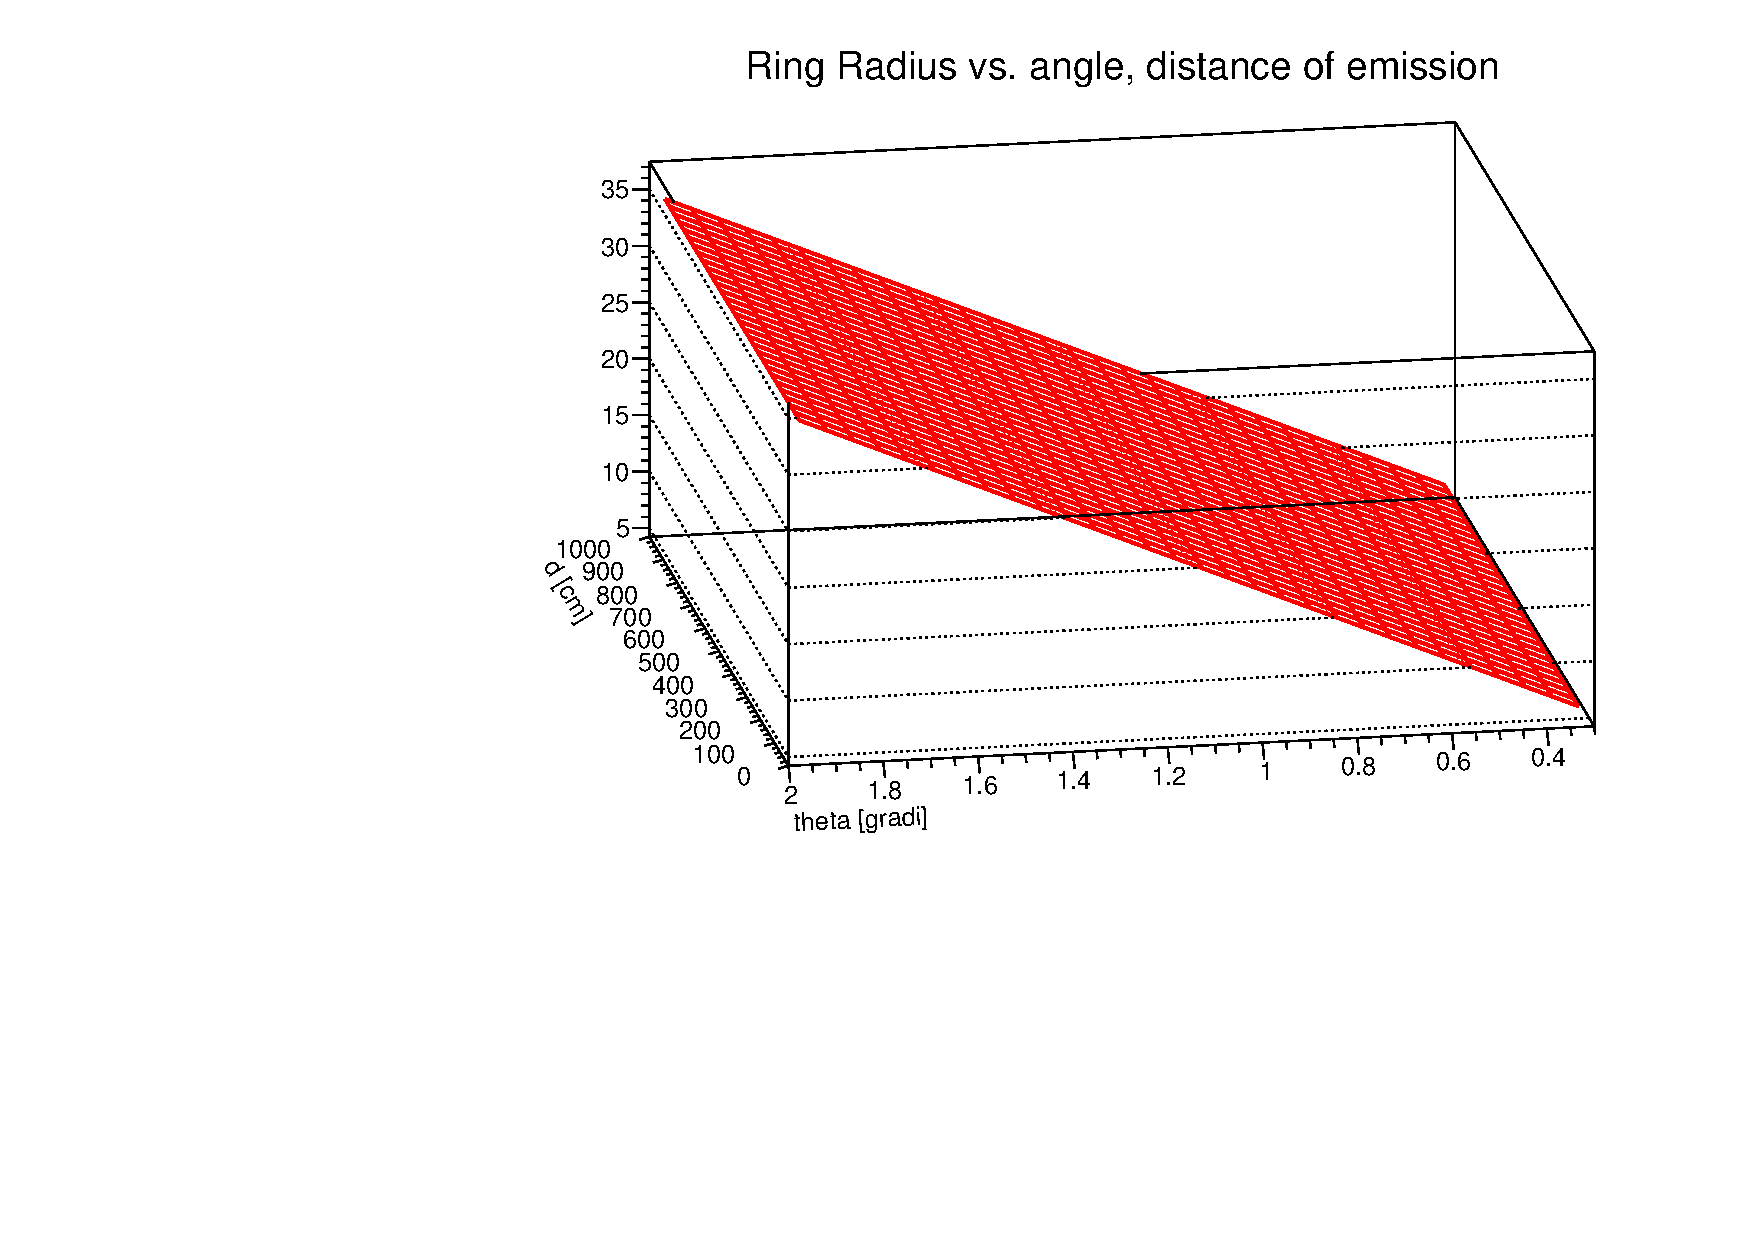
\includegraphics[scale=0.4]{tf2_radius}
\caption{Andamento del raggio in funzione della distanza di emissione rispetto allo specchio e all'angolo di emissione. La distanza massima corrisponde alla dimensione del rivelatore Cerenkov.}
\label{fig:tf2_radius}
\end{center}
\end{figure}

\begin{figure}
\begin{center}
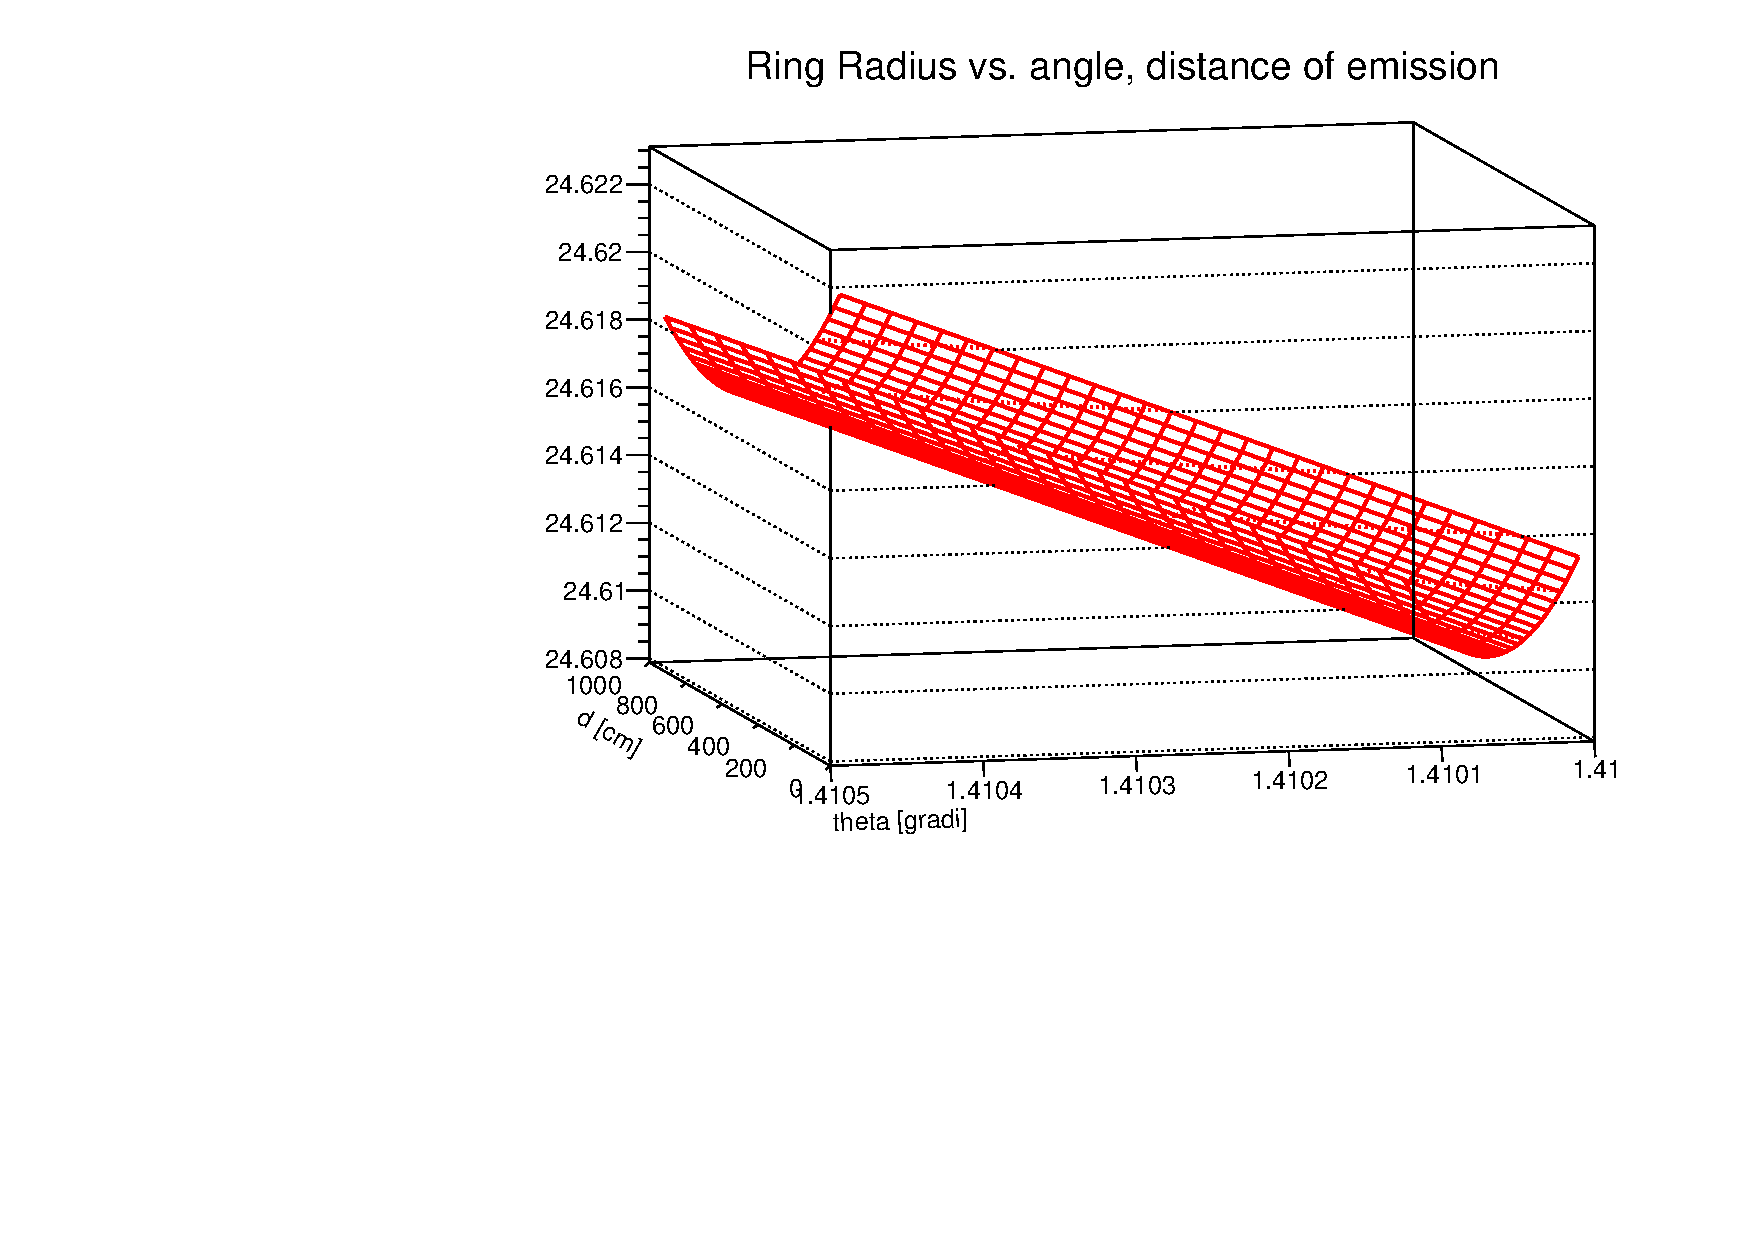
\includegraphics[scale=0.4]{tf2_radius_zoom}
\caption{Zoom della relazione precedente in un intervallo angolare vicino a quello sperimentale del $\pi$.}
\label{fig:tf2_radius_zoom}
\end{center}
\end{figure}

Tale andamento si mostra in ottima approssimazione lineare con l'angolo secondo un coefficiente di proporzionalità pari alla lunghezza focale. Nella figura \ref{fig:tf2_deviazione} è mostrato l'andamento con $\theta$ e $d$ della quantità: $R(\theta,d)-f\theta$. \\

\begin{figure}
\begin{center}
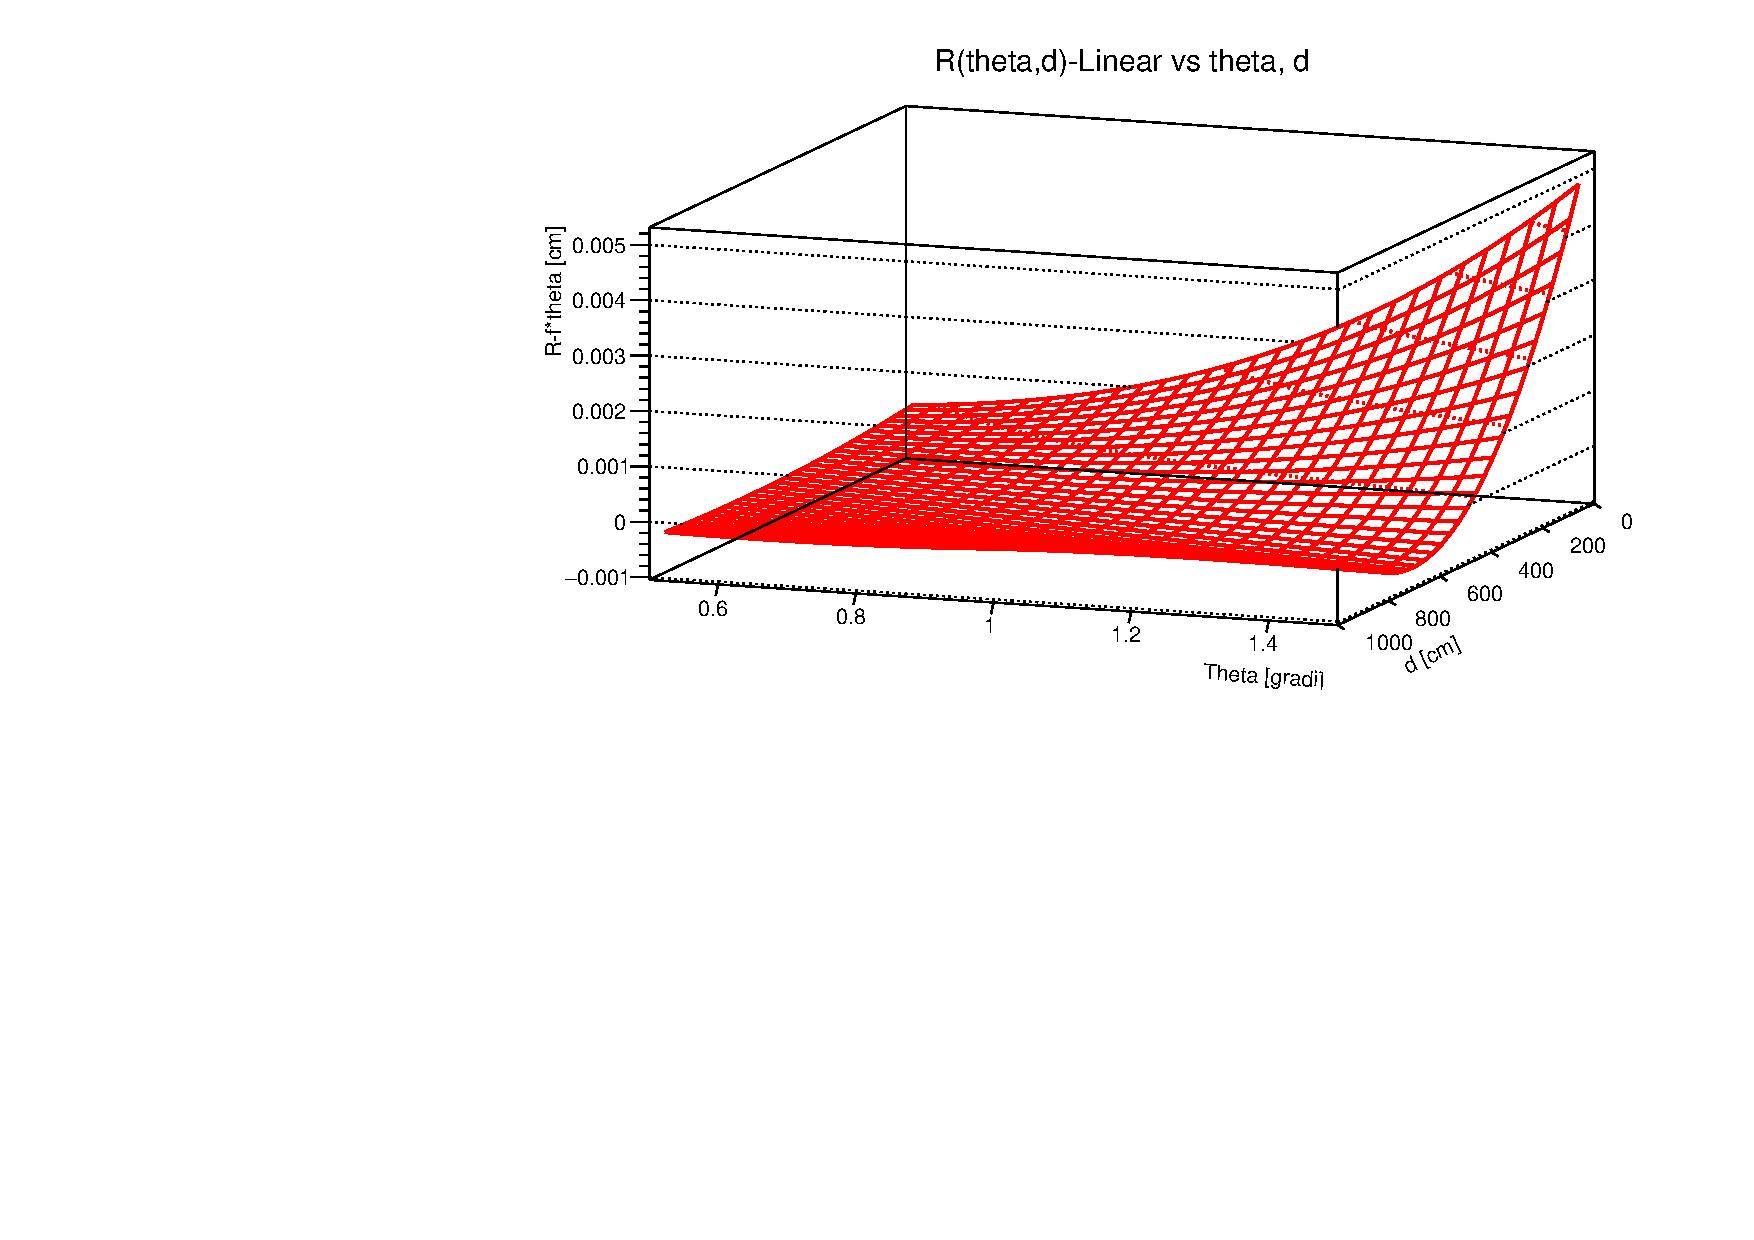
\includegraphics[scale=0.4]{tf2_deviazione}
\caption{Grafico dell'errore commesso utilizzando la relazione lineare in funzione della distanza e dell'angolo di emissione. La distanza massima corrisponde alla dimensione del rivelatore Cerenkov.}
\label{fig:tf2_deviazione}
\end{center}
\end{figure}

A causa della risoluzione sperimentale, ad ogni particella non corrisponde un raggio ben definito, ma una distribuzione la cui deviazione standard potrà essere utilizzata per stimare l'errore. Questa incertezza è stata verificata essere un fattore dieci superiore all'errore commesso trascurando la non linearità in $\theta$ della formula del raggio, rendendo quindi legittimo utilizzare tale approssimazione.

\subsection{Segnale nello scintillatore} \label{sub:scint}
Ad una distanza di 9000 cm dallo specchio parabolico del rivelatore Cerenkov è posto uno scintillatore dalla forma di corona circolare, con $R_{min}=10\ cm$ e $R_{MAX}=100\ cm$, nel quale vengono rivelati i muoni provenienti da eventuali decadimenti delle particelle del fascio.
L'energia di quest'ultimo, unitamente alle dimensioni dell'apparato, fa si tuttavia che i muoni del canale $\pi^+ \ \rightarrow \ \mu^+ \nu_\mu$ non siano rivelati nello scintillatore, passando sempre a una distanza dall'asse del fascio $r<R_{min}$. \\
Infatti, noto l'angolo $\alpha$ con cui il muone viene emesso nel sistema di riferimento a riposo del pione, risulta per l'angolo $\alpha'$ nel sistema del laboratorio:
\begin{equation}
\tan{\alpha}=\frac{p_T}{p_L}
\end{equation}
\begin{equation}
\tan{\alpha'}=\frac{p_T}{p_L'}=\frac{p\sin{\alpha}}{\gamma_{\pi}\big[p\cos{\alpha}+\beta_{\pi} (p^2+m_mu^2)^{1/2}\big]}
\end{equation}
\\
L'andamento della funzione $\alpha'(\alpha)$ è mostrato in [FIGURA], e presenta un punto  di massimo per $	\alpha=105.523°$ $\rightarrow$ $\alpha'=0.0184°$.\\
Un $\pi$ che decadesse all'interno del Cerenkov dopo aver prodotto segnale in esso produrrebbe pertanto un muone che giungerebbe allo scintillatore con una distanza dall'asse di al massimo $r=10000\ cm \cdot \theta (rad) \simeq 3.2 cm$.\\
\\
Gli eventi di $\pi$ saranno dunque caratterizzati dall'assenza di hits nello scintillatore. La proposizione inversa non è invece vera: essendo $\gamma_K \beta c \tau_K \ \sim 900 \ m$, solo una frazione dei K decadrà nei 100 m coperti dall'apparato. Si considera inoltre che il branching ratio del canale di decadimento $K^+ \rightarrow \mu^+\nu_mu$ a cui è sensibile lo scintillatore è $BR_{\mu 2}=63.5\%$, e anche di questi decadimenti una frazione risulterà in muoni che attraversano il foro dello scintillatore, non producendo ugualmente segnale.
\\
\section{Metodo}
Evento per evento sono forniti il numero di hit (0 o 1) registrati nello scintillatore, il numero di pixel della superficie sensibile del rivelatore Cerenkov interessati dall'arrivo di uno o più fotoni e l'identificativo di questi ultimi secondo uno schema a griglia.\\
\subsection{Ricostruzione del raggio dell'anello Cerenkov}
La ricostruzione evento per evento del raggio dell'anello Cerenkov è stata portata a termine seguendo il metodo dei minimi quadrati adattato ad una funzione di fit circolare. La procedura, spiegata in \cite{fit_cerchio}, consiste nell'identificazione di centro e raggio della circonferenza minimizzando la quantità:
\begin{equation}
S=\sum_i g(u_i, v_i, R)^2 \ = \ \sum_i \Big[ (u_i-u_c)^2+(v_i-v_c)^2 - R^2 \Big]
\end{equation}
\\
Dove $u_i, v_i$ rappresentano le coordinate di ciascun pixel di interesse in un sistema cartesiano centrato di volta in volta nella media dei pixel attivi $( \ u_i=x_i-\sum_j x_j /N\ )$. La minimizzazione viene effettuata rispetto ai parametri del fit $u_c, v_c, R$ coordinate del centro del cerchio e raggio di quest'ultimo.\\
\subsection{Frazione di K nel fascio}
Nell'assunto che i raggi degli anelli generati dal passaggio delle due particelle siano distribuiti secondo una Normale con media $\mu_{K,\pi}=\theta_{K,\pi}f$ e varianza determinata dalla risoluzione sperimentale, l'istogramma dei raggi negli eventi disponibili è stato fittato con la somma di due distribuzioni gaussiane con parametri di ampiezza, media e varianza liberi.\\
\\
A partire dai parametri ottenuti ottenuti dal fit il numero di mesoni $K$ e $\pi$ sono stati ottenute integrando separatamente le due distribuzioni appena determinate.\\
\subsubsection{Incertezza su $f_K$} \label{subsub:pseudo}
L'incertezza sulla frazione di K nel fascio è stata calcolata con il metodo degli pseudo esperimenti. Il contenuto di ciascun bin dell'istogramma è distribuito secondo una Binomiale con probabilità di successo della prova stimata in $\hat{p}_i = N_{i}/N$, con $N_i$ contenuto dell'i-esimo bin e N numero totale di eventi. A partire da tale distribuzione il contenuto dei bin è stato fatto variare casualmente, ottenendo così una serie di pseudo distribuzioni di raggi Cerenkov, a loro volta fittate ciascuna con una somma di due gaussiane.\\
La frazione dei mesoni $K$ è stata ottenuta come valor medio della distribuzione di $f_K$ nei vari pseudo esperimenti, e si è utilizzata la deviazione standard di tale distribuzione come incertezza sul valore sperimentale di $f_K$

\subsection{Misura dell'indice di rifrazione}
La relazione (\eqref{eq:raggio_theta}) può essere riformulata in funzione di massa della particella e indice di rifrazione sfruttando l'uguaglianza (\eqref{eq:cerenkov}) e il fatto che $\beta^2=(1+\gamma^{-2})=(1+\frac{m^2}{E^2})$. In questo modo si ottiene una relazione che invertita permette di misurare l'indice di rifrazione in funzione del raggio misurato. Essendo quest'ultimo noto con una data incertezza, anche l'indice di rifrazione avrà una sua incertezza. Quest'ultima è stata calcolata misurando il valore dell'indice di rifrazione al variare del raggio secondo la distribuzione misurata. L'indice di rifrazione può essere calcolato sia a partire dai dati relativi ai mesoni $K$, sia da quelli relativi ai mesoni $\pi$. Essendo il mezzo attraversato dalle particelle lo stesso, si è controllato, per verifica, che i risultati ottenuti nei due modi fossero compatibili.

\subsection{Intervallo di confidenza per l'identificazione dei K}
A causa dell'elevata energia del fascio rispetto alle masse delle due specie di particelle, i $\beta$ dei $\pi$ e dei $K$ sono molto simili, ragion per cui ci si attende un intervallo di raggi per cui esiste una probabilità non trascurabile, date le rispettive distribuzioni, di avere un evento sia di $\pi$ che di $K$.\\
Volendo assicurare una procedura per l'identificazione dei K del fascio con un certa confidenza a discrezione dello sperimentatore, è necessario definire in relazione a tale livello di confidenza un intervallo di valori per il raggio dell'anello rivelato nella camera a gas.\\
Un taglio severo sul raggio dell'anello Cerenkov porta tuttavia non solo ad una forte minimizzazione della probabilità che un evento identificato come $K$ sia in realtà un $\pi$, ma contemporaneamente anche all'aumento della frazione di legittimi eventi di $K$ scartati in quanto fuori dall'intervallo di confidenza. A seconda delle finalità dell'esperimento e dalle esigenze sperimentali si può scegliere un intervallo molto severo che permetta di usare l'apparato come un trigger "purificando" il fascio a scapito della luminosità, o alternativamente un intervallo più lasco, favorendo il numero di eventi totali sulla purezza del fascio.

\subsubsection{Probabilità di identificare un $\pi$ come un K} \label{subsub:mis}
L'estremo inferiore dell'intervallo di confidenza è posto a $R_{min}=\bar{R_K}-4\sigma_K$, con una perdita di eventi di K con $r<\bar{R_K}-4\sigma_K$ pari allo 0.006\%. La probabilità che un evento accettato come K fosse in realtà un $\pi$ è funzione dell'estremo superiore $R_{max}$ dell'intervallo. Ognuna delle probabilità che appaiono nelle equazioni a seguire sono ricavate dal teorema di Bayes. Esse sono calcolate sperimentalmente come un rapporto tra integrali delle distribuzioni sperimentali. Ad esempio, la probabilità che, essendo passato un $K$, esso abbia prodotto un segnale nel rivelatore Cerenkov corrispondente ad un raggio maggiore di $R_{max}$ è semplicemente l'integrale della gaussiana corrispondente al $K$ (estratta dal fit della distribuzione del raggio) calcolato nell'intervallo scelto diviso per il valore dell'integrale totale della stessa gaussiana. Per quanto riguarda le probabilità che riguardano il numero di tracce nello scintillatore si è proceduto in maniera analoga, utilizzando però la gaussiana estratta dalla distribuzione dei soli raggi associati a passaggi di un $\mu$ nello scintillatore. \\
Nel caso in cui l'identificazione del $K$ prescindesse dal numero di tracce nello scintillatore avremmo una probabilità di erronea identificazione: \\

\begin{equation}
P(\pi | R<R_{max})=\frac{P(R<R_{max}|\pi)P(\pi)}{P(R<R_{max}|\pi)P(\pi)+P(R<R_{max}|K)P(K)}
\end{equation}
\\

Nel caso la quantità di interesse fosse la probabilità di identificazione non corretta di un $\pi$ da parte del rivelatore Cerenkov facendo uso di tutti i dati a disposizione, la probabilità va corretta tenendo conto anche di quegli eventi che pur risultando in un $R>R_{max}$ producono un segnale nello scintillatore, escludendo che si tratti di eventi di $\pi$. La probabilità diventa:
\begin{equation}
\begin{split}
&P(\pi | R<R_{max} \cup S = 1) = \\
&\frac{P(R<R_{max}|\pi)P(\pi)}{P(R<R_{max}|\pi)P(\pi)+\left[P(R<R_{max}|K)+P(R>R_{max}|K)P(S=1|K)\right]P(K)} \\
\end{split}
\end{equation}
\\
Se invece l'obiettivo è di produrre un segnale di trigger tramite gli output dello scintillatore e del Cerenkov al fine di selezionare solamente i K in uscita dall'apparato per un utilizzo successivo, si deve tenere conto del fatto che gli eventi con segnale nello scintillatore risultano da un decadimento di un K che non sarà dunque presente in uscita dall'apparato.\\
La probabilità di identificazione non corretta di un K, a parità di $R_{max}$ risulta superiore a causa del minor numero complessivo di eventi accettati con $R<R_{max}$ e risulta:
\begin{equation}
P(\pi | R<R_{max} \cap S=0 )=\frac{P(R<R_{max}|\pi)P(\pi)}{P(R<R_{max}|\pi)P(\pi)+P(R<R_{max}|K)P(S=0 |K)P(K)} 
\end{equation}

\subsubsection{Probabilità di non identificare un K} \label{subsub:nidK}
Definire un intervallo di confidenza per l'accettazione di un evento di K porta in qualunque caso a perdere una frazione di eventi legittimi. Tale frazione risulta, nei tre casi descritti nella sezione precedente:
\begin{equation}
P(R>R_{max}|K)= \frac{\int_{R_{min}}^{R_{max}} \! K}{\int_{0}^{+\infty} \! K}
\end{equation}

\begin{equation}
P(R > R_{max} \cap S = 0 | K) = P(R > R_{max} | K) P(S = 0 | K)
\end{equation}

\begin{equation}
P(R > R_{max} \cup S = 1 | K) = P(R > R_{max}| K) + P(S = 1| K) - P(R > R_{max}| K)P(S = 1| K)
\end{equation}

\section{Risultati}
\subsection{Frazione di K nel fascio}
Per prima cosa si è ricostruita la distribuzione del numero di pixel interessati dall'arrivo di un fotone per evento, come mostrato nella \ref{fig:pixnum_dist}. \\

\begin{figure}
\begin{center}
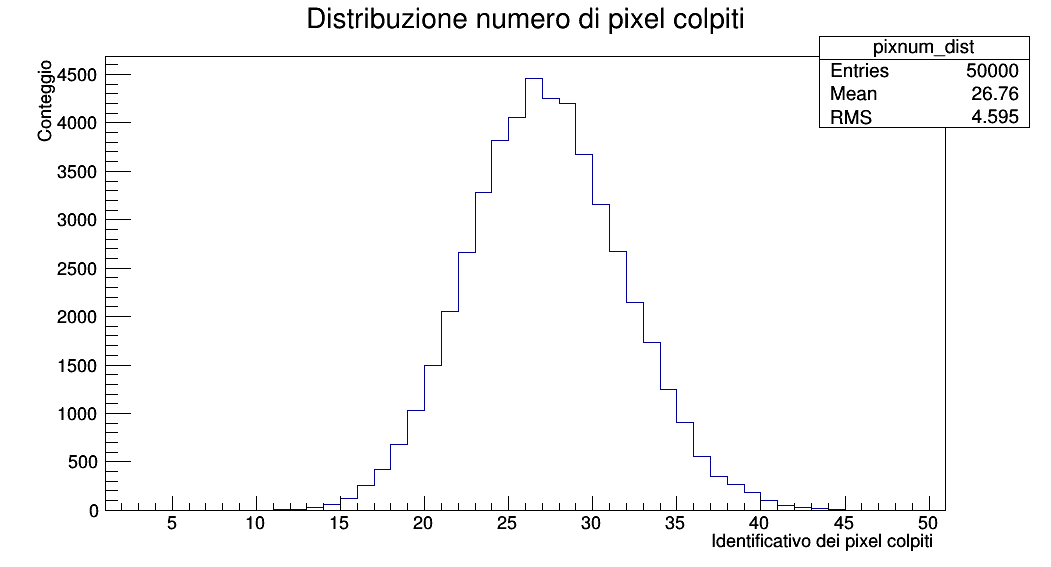
\includegraphics[scale=0.4]{pixnum_dist}
\caption{Distribuzione del numero di tracce nel rivelatore Cerenkov.}
\label{fig:pixnum_dist}
\end{center}
\end{figure}

Le particelle che attraversano la camera a gas rilasciano dunque in media 27 fotoni lungo un percorso di 1000 cm.
\\
Evento per evento si sono determinate le posizioni dei pixel interessati da un evento e a partire da essi si sono determinati i parametri della miglior circonferenza che descrivesse l'evento, secondo l'algoritmo dei minimi quadrati. In fig. \ref{fig:centrox_dist}, \ref{fig:centroy_dist}, \ref{fig:radius_dist} sono mostrate le distribuzioni delle coordinate dei centri e dei raggi nell'arco dei $50\ 000$ eventi disponibili.\\

\begin{figure}
\begin{center}
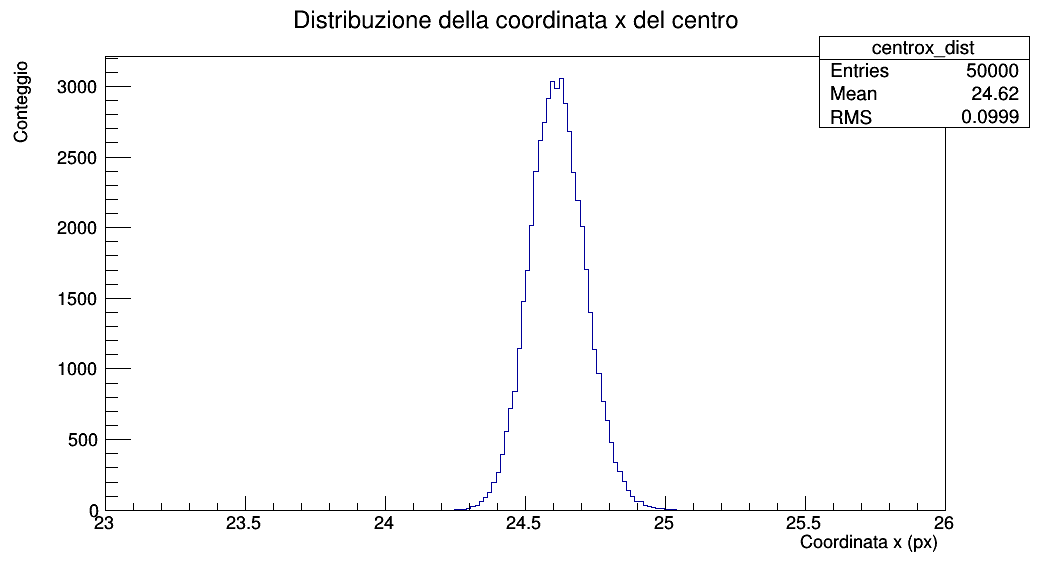
\includegraphics[scale=0.4]{centrox_dist}
\caption{Distribuzione della coordinata x dei centri delle circonferenze fittate.}
\label{centrox_dist}
\end{center}
\end{figure}

\begin{figure}
\begin{center}
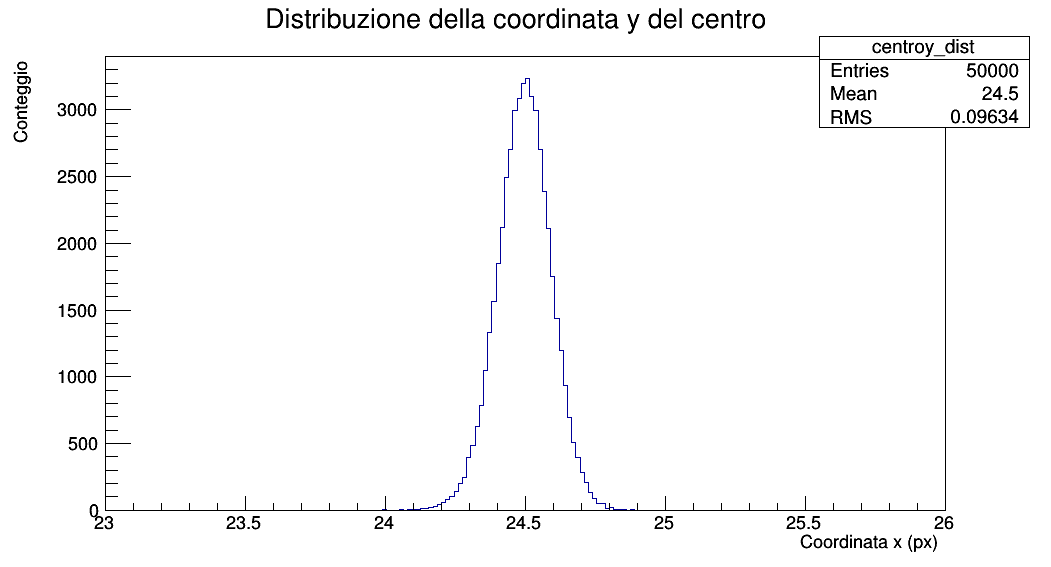
\includegraphics[scale=0.4]{centroy_dist}
\caption{Distribuzione della coordinata y dei centri delle circonferenze fittate.}
\label{centroy_dist}
\end{center}
\end{figure}

\begin{figure}
\begin{center}
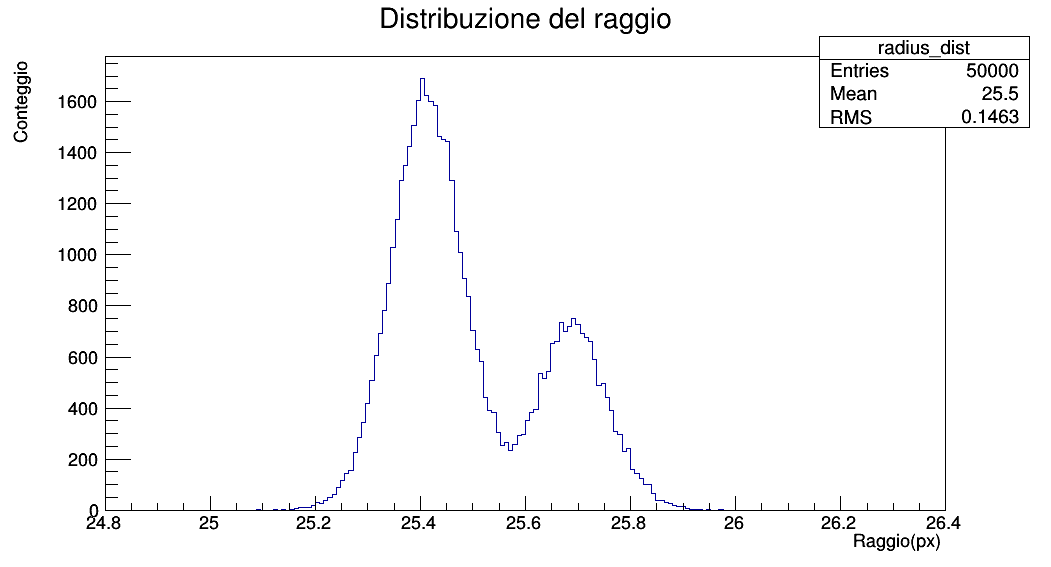
\includegraphics[scale=0.4]{radius_dist}
\caption{Distribuzione dei raggi delle circonferenze fittate.}
\label{radius_dist}
\end{center}
\end{figure}


Si è mostrato nella sezione (\ref{sub:scint}) come i muoni prodotto del decadimento dei $\pi$ non siano in grado di produrre segnale nello scintillatore. La distribuzione dei raggi Cerenkov degli eventi con una traccia nello scintillatore sarà dunque interamente dovuta al passaggio dei mesoni K, sebbene solamente di una frazione di questi. La distrubuzione sperimentale, mostrata in \ref{fig:radius1_dist}, presenta una prova a sostegno di questo modello, non essendo presente un picco in corrispondenza del raggio Cerenkov previsto per un $\pi$. \\

\begin{figure}
\begin{center}
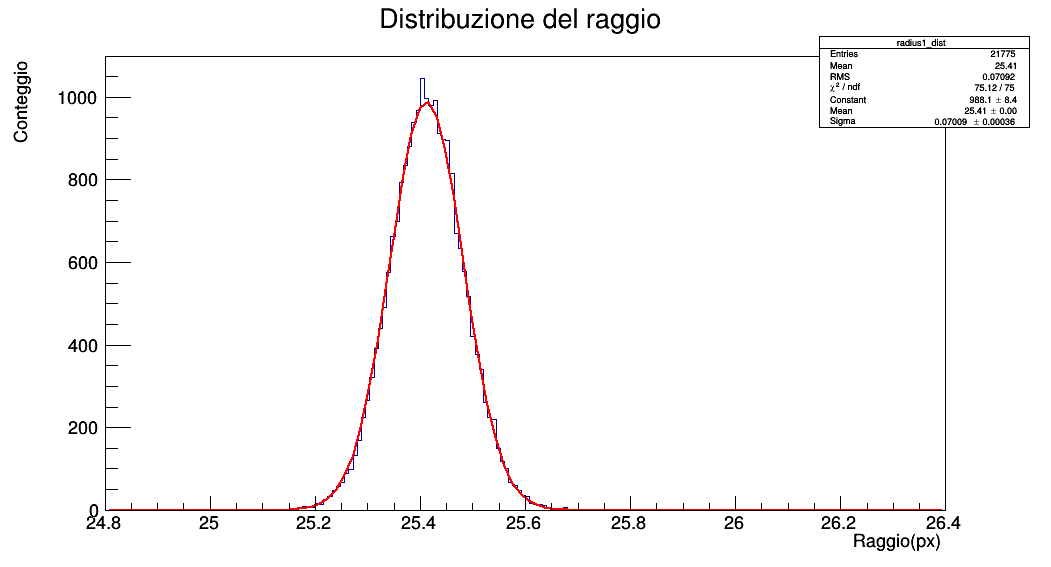
\includegraphics[scale=0.4]{radius1_dist}
\caption{Distribuzione dei raggi delle circonferenze fittate nei casi corrispondenti a una traccia nello scintillatore. Nella figura è anche rappresentato il risultato di un fit gaussiano eseguito sulla distribuzione.}
\label{radius1_dist}
\end{center}
\end{figure}

A partire dalla distribuzione dei raggi dei K che producono segnale nello scintillatore, e tenendo conto che la probabilità di questi ultimi di decadere e di produrre segnale nello scintillatore è la medesima per ogni K, è possibile, mediante un fit, estrarre i parametri di media e varianza dalla distribuzione e utilizzare questi ultimi come parametri fissati per il fit della distribuzione complessiva dei raggi Cerenkov, aumentando così i gradi di libertà del fit.
[TABELLA]
\\
Coerentemente con le previsioni, la distribuzione dei raggi di tutti gli eventi registrati nel rivelatore Cerenkov è una somma di due distribuzioni a campana parzialmente sovrapposte. \'E possibile eseguire un fit utilizzando come funzione di prova la somma di due gaussiane, ricavare le frazioni relative dei due tipi di particelle integrando le singole gaussiane con i parametri stimati dal fit, normalizzando poi sul numero totale di eventi.\\
I risultati del fit e gli integrali delle singole distribuzioni ricostruite sono mostrati nelle tabelle:
[TABELLE]
\subsubsection{Incertezza su $f_K$}
Sono stati effettuati $100\ 000$ pseudo esperimenti di misura della frazione dei mesoni K del fascio, facendo variare il contenuto di ciascun bin dell'istogramma ricostruito dei raggi nel rivelatore Cerenkov secondo la rispettiva distribuzione Binomiale, come mostrato nella sezione (\ref{eq:cerenkov}).\\
La distribuzione della frazione di K $f_K$ ottenuta nel corso di ciascuno pseudo esperimento è mostrata nella [FIGURAAAAA]. \\
La larghezza della distribuzione di $f_K$, assunta Normale e fittata di conseguenza, viene utilizzata come incertezza sulla determinazione sperimentale di $f_K$.
[MAGARI TABELLA]
\subsection{Indice di rifrazione}
Le fig. \ref{fig:indiceK} e \ref{fig:indicePI} riportano le distribuzioni dell'indice di rifrazione ottenute tenendo conto delle distribuzioni dei raggi. Risulta: \\

\begin{figure}
\begin{center}
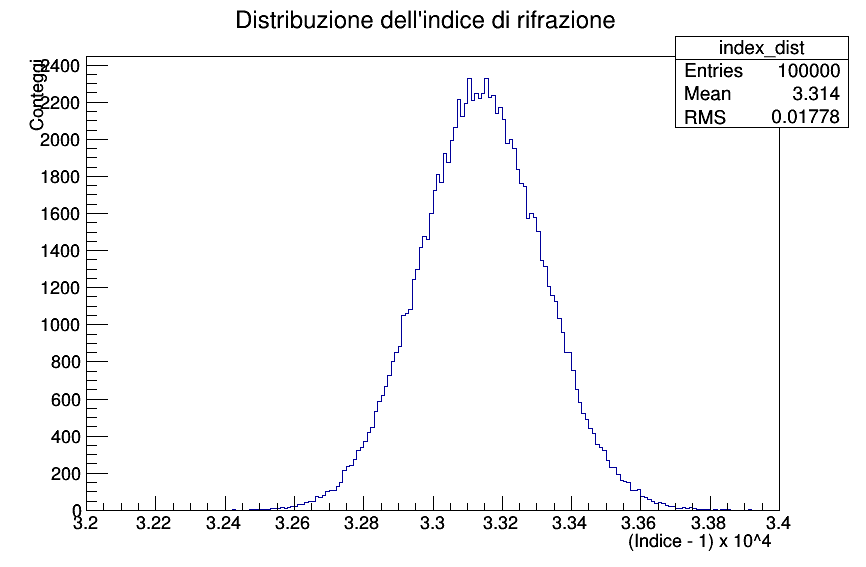
\includegraphics[scale=0.4]{indiceK_definitivo}
\caption{Distribuzione dell'indice di rifrazione ottenuto utilizzando la distribuzione dei raggi associati al passaggio di un mesone $K$.}
\label{fig:indiceK}
\end{center}
\end{figure}

\begin{figure}
\begin{center}
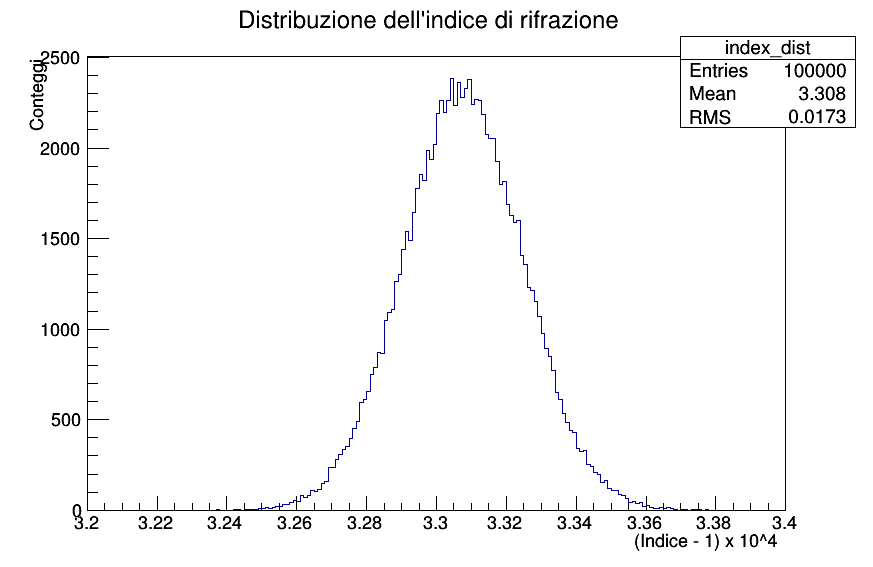
\includegraphics[scale=0.4]{indicePI_definitivo}
\caption{Distribuzione dell'indice di rifrazione ottenuto utilizzando la distribuzione dei raggi associati al passaggio di un mesone $\pi$.}
\label{fig:indicePI}
\end{center}
\end{figure}

I risultati sono quindi perfettamente compatibili: \\
\begin{equation}
n_K -1 = (3.31 \pm 0.02) \cdot 10^{-4}
\nonumber
\end{equation}

\begin{equation}
n_{\pi} -1 = (3.31 \pm 0.02) \cdot 10^{-4}
\nonumber
\end{equation}

\subsection{Intervallo di confidenza}
L'andamento in funzione dell'estremo superiore dell'intervallo di confidenza delle due tipologie di errore illustrate nelle sezioni \ref{subsub:nidK} e \ref{subsub:mis} è rappresentato nelle figure sottostanti nei tre diversi casi trattati:
[FIGURE CON CAPTION]
\\
In ciascuna di essere starà allo sperimentatore determinare il migliore valore di $R_{max}$ relativamente alle esigenze sperimentali contingenti.

\section{Conclusioni}
Una migliore identificazione delle due specie di particelle può essere senz'altro compiuta migliorando la risoluzione dello schermo (ovvero aumentando il numero di pixel in cui esso è suddiviso). Questo è limitato sia da aspetti tecnologici (i pixel non possono essere piccoli arbitrariamente) che dai maggiori costi dell'apparato che ne conseguono. Un altro modo potrebbe essere quello di aumentare le dimensioni del rivelatore (modificando di conseguenza la geometria della parabola in modo che il piano focale risieda alla fine del rivelatore Cerenkov. Nuovamente questo aumenta i costi dell'esperimento e richiede maggiore precisione nell'allineamento del fascio con l'asse della parabola. Al fine di migliorare l'identificazione con l'uso dello scintillatore si può pensare di aumentare la sua distanza dal rivelatore Cerenkov, sempre assicurandosi che per i $\mu$ prodotti dai $\pi$ sia impossibile raggiungere lo scintillatore. In questo modo si dà più tempo ai $K$ di decadere e questo aumenta il numero di tracce viste dallo scintillatore, migliorando la probabilità di erronea identificazione. Questo non vale nel caso in cui l'identificazione sia condotta con il terzo metodo (con riferimento alla sez. \ref{subsub:mis}).

\input{bibanalisi.bib}


\end{document}
